% Template for ICASSP-2018 paper; to be used with:
%          spconf.sty  - ICASSP/ICIP LaTeX style file, and
%          IEEEbib.bst - IEEE bibliography style file.
% --------------------------------------------------------------------------
\documentclass{article}
\usepackage{spconf,amsmath,graphicx}

% Example definitions.
% --------------------
\def\x{{\mathbf x}}
\def\L{{\cal L}}

% Title.
% ------
\title{SEMI-SUPERVISED LEARNING WITH DEEP NEURAL NETWORKS FOR RELATIVE TRANSFER FUNCTION INVERSE REGRESSION }
%
% Single address.
% ---------------
%\name{Author(s) Name(s)\thanks{Thanks to XYZ agency for funding.}}
%\address{Author Affiliation(s)}
%
% For example:
% ------------
%\address{School\\
%	Department\\
%	Address}
%
% Two addresses (uncomment and modify for two-address case).
% ----------------------------------------------------------
\twoauthors
  {Ziteng Wang\sthanks{Thanks to CSC (201604910623) for funding. The work was performed while the author was at Inria.}, Yonghong Yan}
	{University of Chinese Academy of Sciences\\
	Institute of Acoustics\\
	Beijing, China}
  {Emmanuel Vincent}
	{Inria\\
	Villers-l{\`e}s-Nancy, France}
%
\begin{document}
\ninept
%
\maketitle
%
\begin{abstract}
The prior knowledge of relative transfer function (RTF) is preferable in many applications but remains less studied. In this paper, we propose a semi-supervised learning algorithm based on deep neural networks (DNNs) for RTF inverse regression, that is to generate the full-band RTF vector directly from the source-receiver \emph{pose} (position and orientation). Two typical scenarios are discussed: training on labeled RTFs with or without unlabeled ones. Both setups utilize the low-dimensional manifold property of RTF in stationary environments. With this property as an additional regularization term, a smooth mapping solution with respect to the manifold is obtained. Experimental simulations show that the proposed method achieves lower mean prediction errors than the free field model with few labeled RTFs, and the unlabeled ones are essential in improving the inverse regression performance.
\end{abstract}
%
\begin{keywords}
relative transfer function, semi-supervised learning, deep neural network, manifold regularization
\end{keywords}
%
\section{INTRODUCTION}
\label{sec:intro}

% v 1: background -> RTF->AIR modeling -> Supervised -> Semi-supervised
% v 2: background -> Supervised -> Semi-supervised

Relative transfer function (RTF)~\cite{gannot2001signal,cohen2004relative} represents the coupling between a pair of microphones in response to the source signal. The estimation of RTF has been an essential task in many applications, such as beamforming~\cite{talmon2009relative}, source separation~\cite{taseska2015relative} and  source localization~\cite{li2015estimation}. Generally the estimation is based merely on the microphone observations, and the prior knowledge of RTF given the source-microphone pose remains less studied. Such knowledge could bring additional performance benefits~\cite{talmon2013relative,koldovsky2013semi}.

The RTF relates two acoustic transfer functions (ATFs) and hence depends on the properties of the acoustic environment and on the poses of the source and microphones. Conventional room acoustic simulation methods, such as the image-source method~\cite{allen1979image}, rely on explicit physical models to simulate the ATF. Recent practices perform transfer function interpolation based on models derived from the wave propagation equation~\cite{samarasinghe2015efficient,mignot2014low}. In~\cite{rtfinv2017}, we proposed to predict the full-band RTF vector from a distinctive data-driven perspective, which was defined as RTF inverse regression. A deep neural network (DNN) model was trained to learn the mapping from the low-dimensional source pose to the high-dimensional RTF based on pairwise data collected in advance. It turned out that with enough dense training samples, a simple linear interpolation~\cite{vincent2013second} could also achieve low mean prediction errors.

Imagine the scenario that a smart device collects data automatically in the environment, as what could happen, e.g., in conference rooms or cars. Labeling the data to obtain enough pairwise training samples can be a cumbersome task, and this motivates the semi-supervised learning setup in this paper. To train on the unlabeled RTFs, we propose an \emph{encoder-decoder} framework and utilize the low-dimensional manifold property of RTF that was discussed recently in the source localization tasks~\cite{deleforge20122d,laufer2013relative,deleforge2015acoustic,laufer2016mr}. A smoothness constraint on the manifold is introduced to regularize the encoder network, which first gives the RTF noisy labels. The function and necessity of the unlabeled RTFs are further investigated in experimental simulations. The results show that the performance degrades with few labeled data compared to the fully labeled case, but the unlabeled samples are indispensable in the inverse regression performance.

\section{DEFINITIONS}
\label{sec:defs}

In a standard enclosure, an unknown signal $S$ is emitted from the source and measured by a pair of microphones. For simplicity, the microphones are assumed to be fixed and the source pose is given by ${\bf p}=[\rho,\theta,\phi]$, the spherical coordinates. Under the narrowband approximation, the observations in the short-time Fourier transform (STFT) domain are written as
\begin{equation}\label{eq:sigfreq}
  A_m(n,k) = H_m({\bf p},k)S(n,k) + V_m(n,k), ~~m=1,2
\end{equation}
where $n$ denotes the time index and $k$ denotes the frequency index, $H_m$ is the acoustic transfer function relating the source and the $m$th microphone and $V_m$ is the additive noise. The RTF is defined as
\begin{equation}\label{eq:rtf}
  H({\bf p}, k) = \frac{H_2({\bf p}, k)}{H_1({\bf p}, k)}.
\end{equation}

The RTF is first independent of the source signal, and in stationary environments the source pose is the only factor that controls its variations. For instance, this association is given by
\begin{equation}\label{eq:green}
  H_d({\bf p},k)={\text{exp}(j\cdot 2\pi k \frac{|r_2({\bf p}) - r_1({\bf p})|}{c})}
\end{equation}
under the free field assumption, where $j$ is the complex unit, $c$ denotes the speed of sound and $r_{2}, r_{1}$ are the Euclidean distances between the source and the microphones. In reverberant conditions, the association becomes complex due to the effect of multi-path propagation. The RTF inverse regression is then to predict the full-band RTF from the source-microphone pose based on pre-collected training examples. For clearness, the RTF is referred as \emph{sample} and the pose as \emph{label} in the following.


\section{RELATION TO PRIOR WORK}

In~\cite{deleforge2015acoustic}, probabilistic piecewise affine mapping (PPAM) realized a bijective mapping between the interchannel level difference (ILD) and interchannel phase difference (IPD) vector and the source-receiver pose. ILD and IPD are defined by $\text{ILD}({\bf p}, k)=20{\rm log}_{10}|H({\bf p}, k)|$ and $\text{IPD}({\bf p}, k)={\rm arg}(H({\bf p}, k))$, respectively, that are equivalent representations of RTF. Nevertheless, this method was only discussed for source localization. In~\cite{rtfinv2017}, we evaluated PPAM in terms of RTF inverse regression performance together with linear interpolation and our proposed DNN model, which were all supervised setups. We briefly review this work as follows.

Given pairwise training RTFs and poses, the DNN model is optimized to minimize the mean squared prediction error:
\begin{equation}\label{eq:Dmmse}
  \text{MSE} = \sum_{i}||\mathcal{D}({\bf p}_i) - {\bf h}_i||^2
\end{equation}
where $\mathcal{D}({\bf p}_i)$ is the model output from input pose ${\bf p}_i$. Since the RTF is complex value, the target vector ${\bf h}_i$ is defined as a concatenation of $\text{ILD}({\bf p}, k)$ and the sine and cosine of $\text{IPD}({\bf p}, k)$ in all frequencies. The output nodes corresponding to the sine part $o_{k,s}$ and cosine part $o_{k,c}$ are thus normalized by
\begin{equation}\label{eq:ln}
  o_{k,s/c}=\frac{o_{k,s/c}}{\sqrt{o_{k,s}^2+o_{k,c}^2}}
\end{equation}
that ensures their squared sum to be one. This model is illustrated by the $decoder$ network in Fig.~1(c). In the test phase, the trained decoder is used to generate RTF of a new pose ${\bf p}_t$ as $\widehat{{\bf h}_t}=\mathcal{D}({\bf p}_t)$.


\section{SEMI-SUPERVISED RTF INVERSE REGRESSION}

% why ILD/IPD
The semi-supervised setup considers the case that there are only $L$ labeled samples $\{{\bf h}_{1:L}, {\bf p}_{1:L}\}$ and the remaining samples $\{{\bf h}_{L+1:L+U}\}$ are unlabeled. To utilize the unlabeled samples in the training process, an intuitive encoder-decoder architecture is first discussed in Section 4.1. The idea is refined in Section 4.2 by optimizing the encoder network with manifold regularization, which turns out in latter experiments as giving the unlabeled RTFs noisy pose labels. An illustration of the involved architectures is given in Fig.~1. The network training details are discussed in Section 4.3.

\begin{figure}[tb]
    \centering
    \centerline{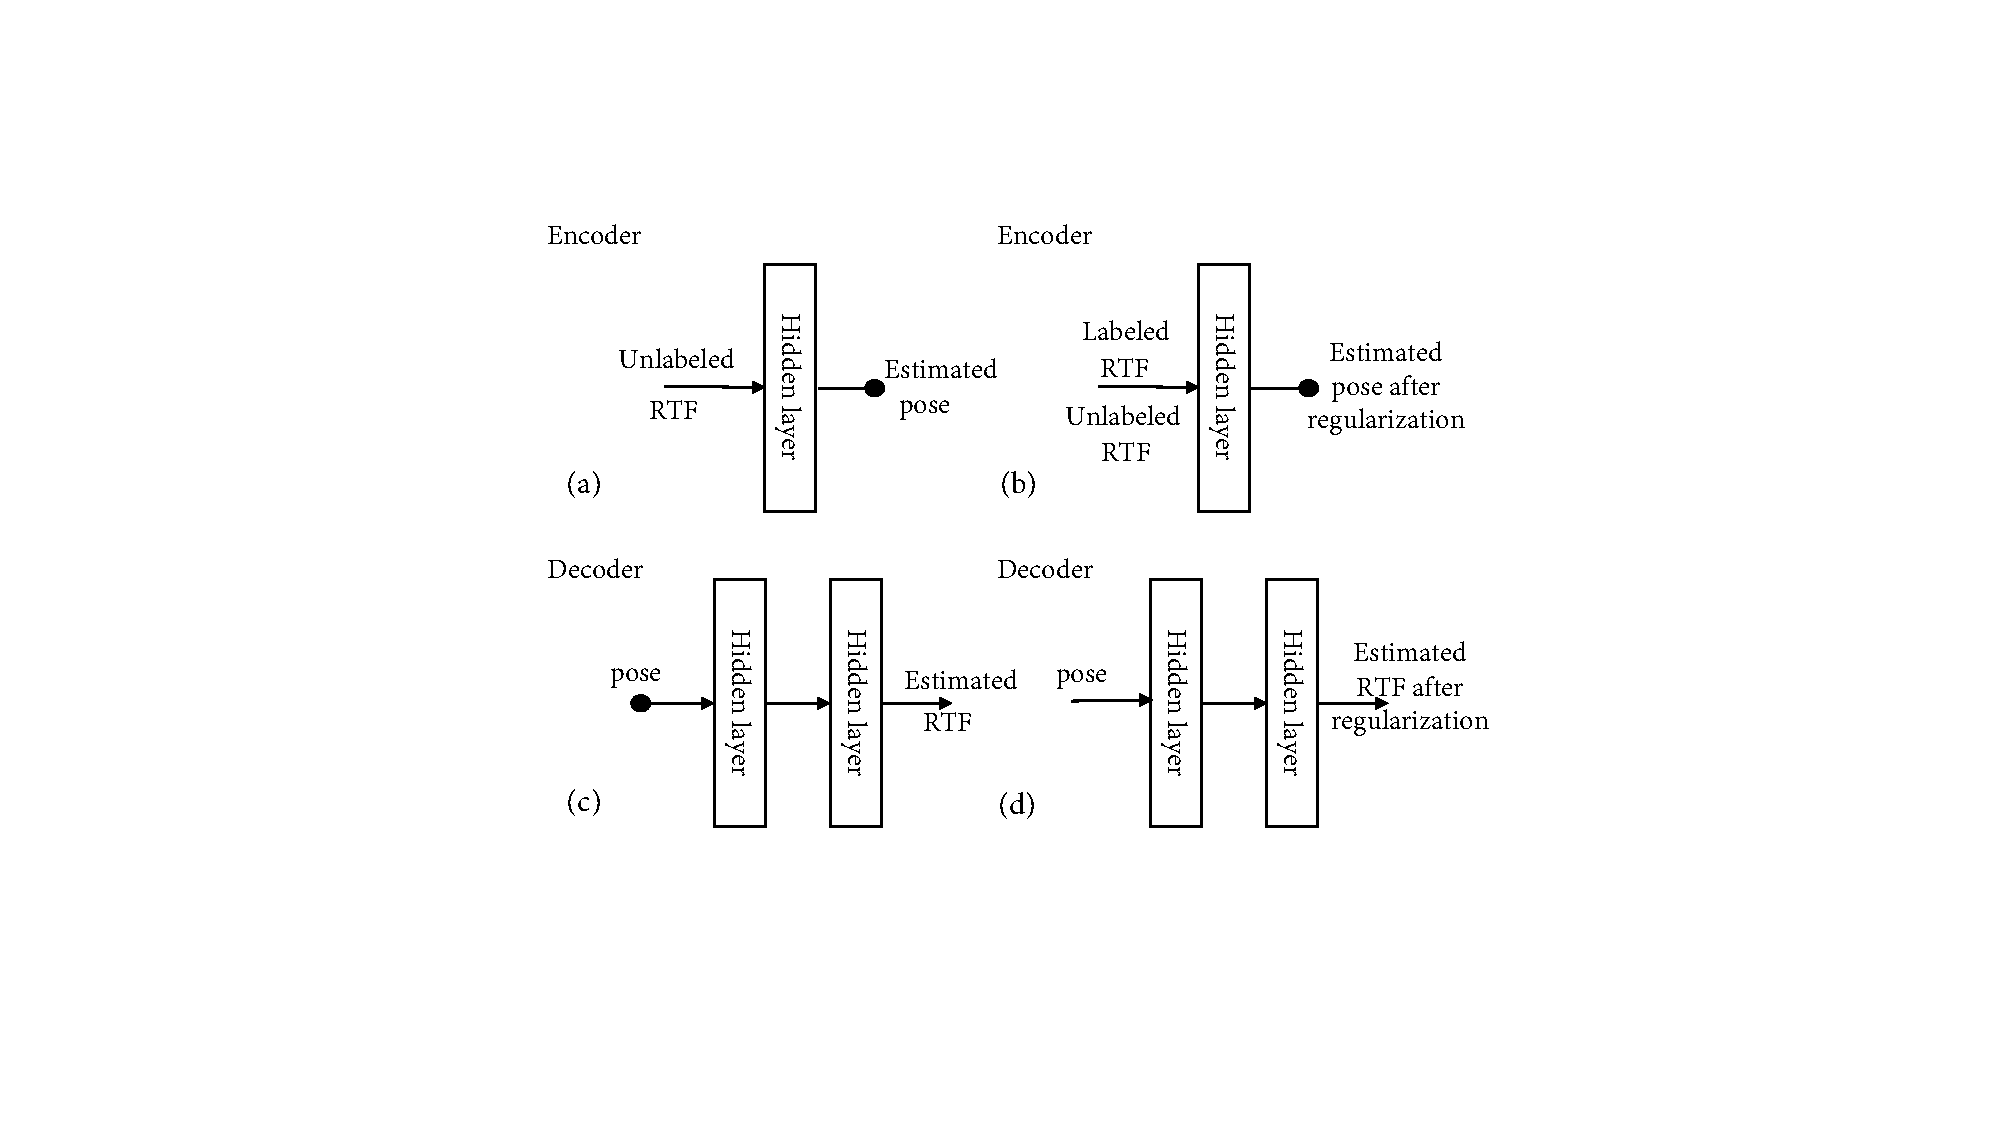
\includegraphics[width=8.3cm]{fig1_nn.pdf}}
    \caption{The encoder and decoder networks proposed for semi-supervised RTF inverse regression.}
    \label{fig1}
\end{figure}

\subsection{Encoder-decoder}

An auxiliary encoder network $\mathit{E}$ is introduced to help optimize the decoder network under the new loss function:
\begin{equation}\label{eq:lossed}
\sum_{i=1}^{L}||\mathcal{D}({\bf p}_i)-{\bf h}_i||^2 + \alpha \sum_{j=1}^{L+U}||\mathcal{D}(\mathit{E}({\bf h}_j))-{\bf h}_j||^2
\end{equation}
where $\alpha$ is a constant scaling factor, and the second term is the reconstruction error on the training samples. This network architecture is given in Fig.~1 by (a)+(c). The encoder can be interpreted as a localization network, that maps the RTF space to the pose space, and the encoder is expected to learn the pose labels implicitly. In the training phase, the encoder and decoder parameters are updated simultaneously.

\subsection{Encoder with manifold regularization}

The work of manifold regularization for localization (MRL)~\cite{laufer2016mr} shows that, the RTFs collected in a specific environment are confined to a low-dimensional manifold with local linearity. A simple validation of this concept is shown in Fig.~2, that plots the Euclidean distances between the RTFs with respect to the pose distances to an arbitrary chosen reference source pose. In a local range of the reference pose (about 1.6$^\circ$ in azimuth and elevation angles as in this case), the distance changes between the corresponding RTFs are approximately linear and uniform in different directions. In other words, a small shift in the source pose only lead to small changes in the RTF and vice versa. The detailed setup can be found in the experiment section.

Inspired by this property, the encoder is further refined from a localization perspective under the loss function:
\begin{equation}\label{eq:lossmr}
\sum_{i=1}^{L}||\mathit{E}({\bf h}_i)-{\bf p}_i||^2 + \beta \sum_{i,j}^{L+U}W_{ij}||\mathit{E}({\bf h}_i)-\mathit{E}({\bf h}_j)||^2
\end{equation}
that incurs a weighted penalty when similar inputs have different outputs. $\beta$ is a scaling factor and the second term is commonly known as graph Laplacian regularization~\cite{Yang2016Revisiting}, that imposes a smoothness constraint on the final mapping solution. $W_{ij}$ is the weight that reflects the adjacency between encoder inputs ${\bf h}_i$ and ${\bf h}_j$, and it is close to 0 when the samples are far away in distance. The standard Gaussian kernel function is then used for weight calculation as in~\cite{laufer2016mr}, since it is symmetric positive semi-definite and meets the locality requirements:
\begin{equation}\label{eq:wij}
  W_{ij} = \exp(-\frac{||{\bf h}_i-{\bf h}_j||^2}{\varepsilon^2})
\end{equation}
where the variance $\varepsilon^2$ controls how fast the value decays with distance. Accordingly, the new encoder-decoder architecture is given in Fig.~1 by (b)+(c). The model is optimized under losses (\ref{eq:lossed}) and (\ref{eq:lossmr}).

\begin{figure}[tb]
    \centering
    \centerline{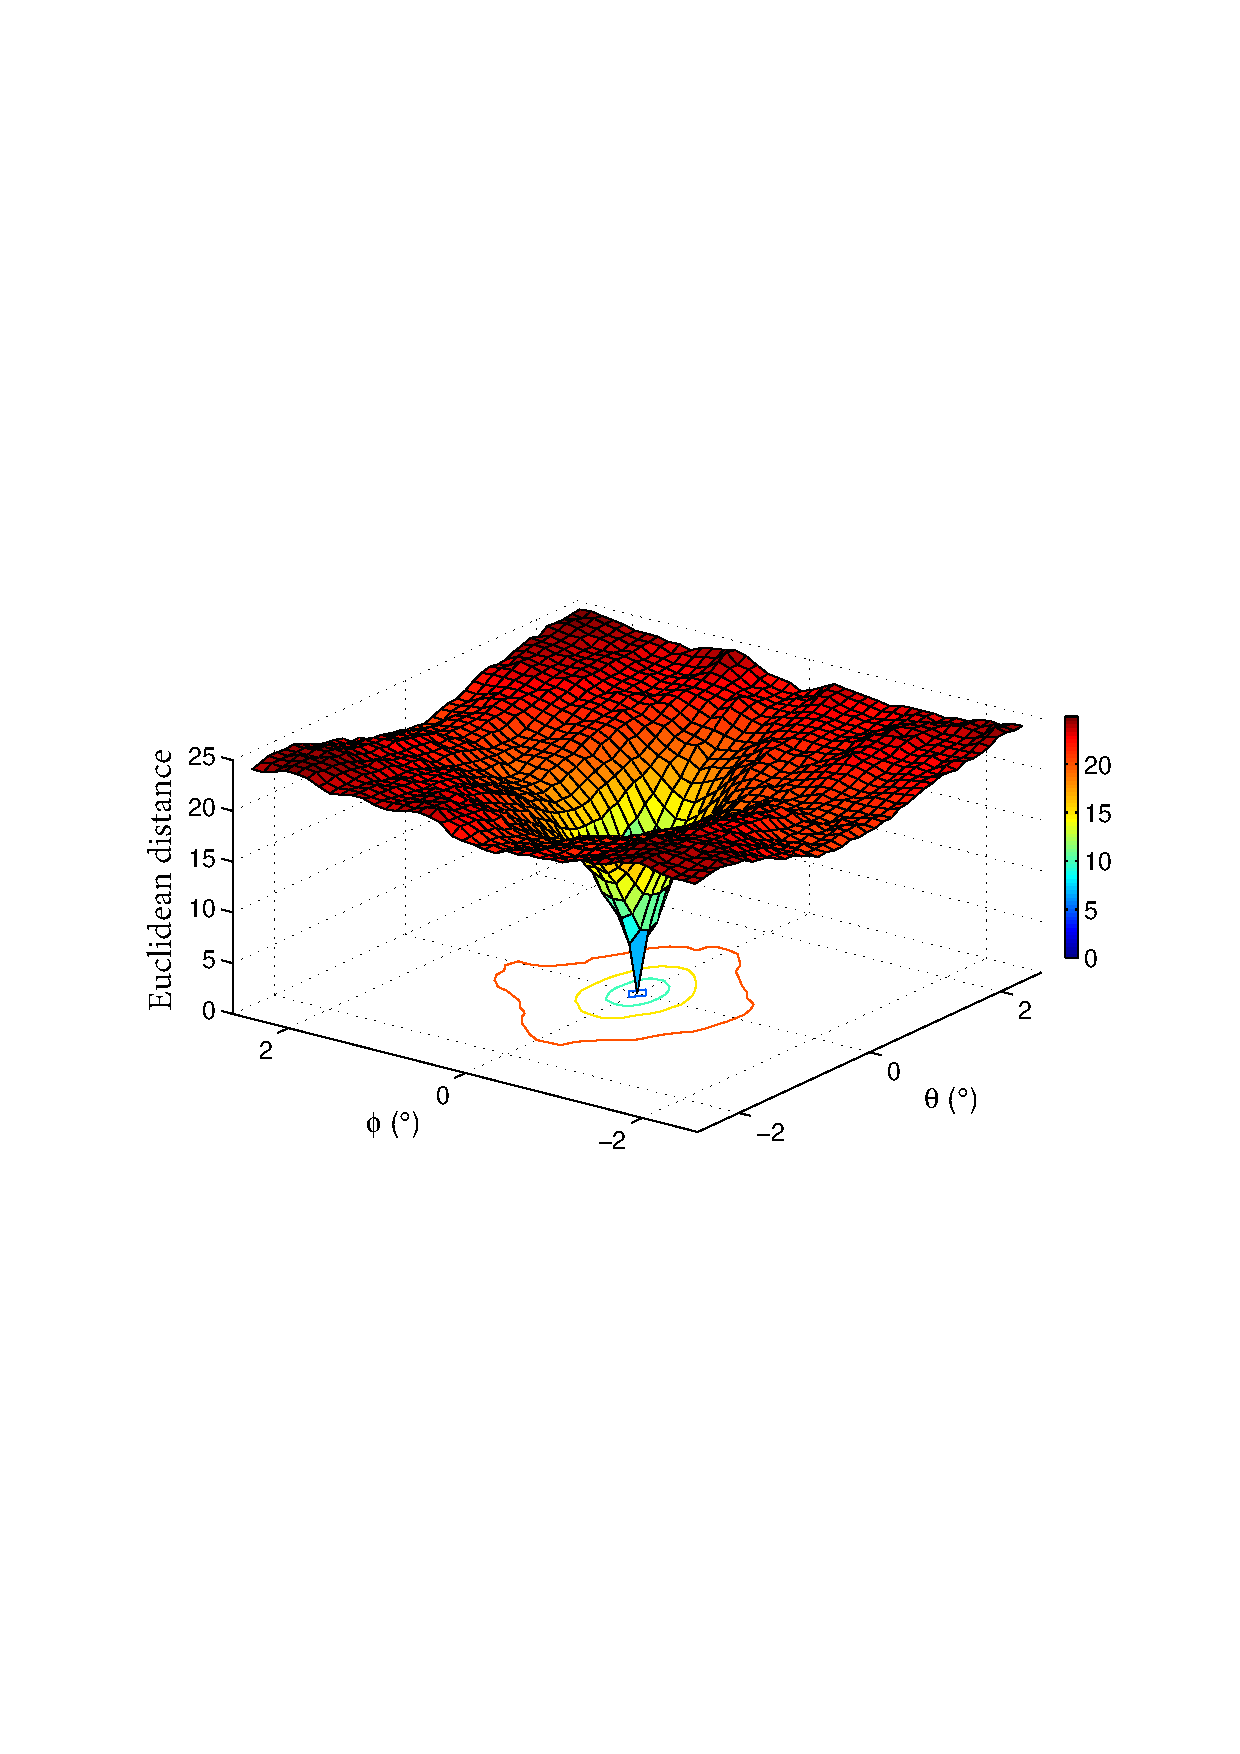
\includegraphics[width=8.0cm]{fig2_euc.pdf}}
    \caption{The Euclidean distances between RTFs with respect to the pose distances to a reference pose.}
    \label{fig2}
\end{figure}

\subsection{Network training}

During training, the networks are initialized following a standard procedure, i.e., the weights are initialized with Gaussian distributed samples and the biases with zeros. ReLU is used as the activation function for all the hidden layers and layer normalization~\cite{ba2016layer} is applied to regularize the parameters. The Adam method~\cite{kingma2014adam} is chosen to update the model using an adaptive learning rate.

One issue with the mini-batch based gradient descent is that the regularization in (\ref{eq:lossmr}) will tend to fail after random shuffling because of the sparse affinity inside the mini-batches, especially with large amount of training data. In~\cite{th2017acoustic}, one nearest-neighbor graph based solution was discussed to sample the data efficiently. We here, however, adopt a simplified technique. The training samples are first randomly shuffled. We then start from one sample, collect all its neighbors, move on to the next remaining sample and repeat until the mini-batch size is reached. The regularization is found to gradually take place against all the adjacent samples after several training epoches.

For the refined encoder, the network is first trained and then kept fixed when the decoder is optimized under loss (\ref{eq:lossed}), while further joint tuning doesn't bring additional performance gains in our case.


\section{Alternative decoder with regularization}


Given the locality property on the RTF manifold as discussed in Section 4.2, we are also motivated to apply regularization directly to the decoder. Since the source poses come free in the environment, there would be even no need to collect the unlabeled RTFs in this case. Similar to (\ref{eq:lossmr}), the loss function for the new decoder network can be defined by

\begin{equation}\label{eq:lossdr}
\sum_{i=1}^{L}||\mathcal{D}({\bf p}_i)-{\bf h}_i||^2 + \gamma \sum_{i,j}^{L+U}w_{ij}||\mathcal{D}({\bf p}_i)-\mathcal{D}({\bf p}_j)||^2
\end{equation}
where $\gamma$ is a scaling factor, and the weight is decided by the pose distances
\begin{equation}\label{eq:wij2}
  w_{ij} = \exp(-\frac{||{\bf p}_i-{\bf p}_j||^2}{\epsilon^2})
\end{equation}
with variance $\epsilon^2$. This decoder is illustrated by Fig.~1(d).


\section{EXPERIMENTS AND ANALYSIS}

\subsection{Setup}

%The experiments are conducted in a simulated setup that is summarized in Table 1.

The experiments are conducted in a simulated room with dimension 6$\times$6.2$\times$3 m and moderate reverberation time 300 ms. Two microphones are positioned at (3,3,1) m and (3.2,3,1) m respectively. The source pose is confined to a spatial area of distance $\rho=2$ m, azimuth angle $\theta \in$[10$^{\circ}$,~60$^{\circ}$], and elevation angle $\phi \in$[0$^{\circ}$,~30$^{\circ}$]. Within this source space, 8 poses are sampled uniformly per degree. For each pose, a one-second white noise signal is emitted from the source and captured by the microphones. The sampling rate is 16 kHz. The corresponding acoustic impulses responses are simulated using an efficient implementation of the image-source method~\cite{rirge}. STFT is applied with frame length 64ms and 87.5\% overlap. The target RTF is then estimated by $\widehat{H}({\bf p}, k)=\frac{\sum_n A_2(n, k)A_1^*(n, k)}{\sum_n |A_1(n, k)|^2}$ with $*$ denoting complex conjugate. Note that the approach here serves as one possible way to measure the RTF in advance, and the white noise signal is special here to provide a reliable estimation in all frequencies.

In total, 400$\times$240 training samples are generated, of which only 24 RTFs are labeled with their true source poses, creating a grid of 10$^\circ$ in angle distance. The input to the decoder network is the source pose ${\bf p}$, and the training target vector is the concatenation of ILD and IPD as discussed in Section 3. We use two hidden layers each with 1024 nodes for the decoder and one hidden layer with 1024 nodes for the auxiliary encoder. The scaling factors $\alpha,~\beta,~\gamma$ are heuristically set to be 0.01. The variances $\varepsilon^2,~\epsilon^2$ are decided such that the weights of samples farther than $2^\circ$ away are close to 0.
%The development set? how to know when to stop training?

For evaluation, 1000 extra poses are picked randomly in the specified source area. As far as we know, there is no established methods to measure closeness of two high-dimensional vectors, and a mean absolute error metric is chosen here to measure the performance, which shows the prediction errors in each frequency:
\begin{equation}\label{eq:err}
  \mu_k = \frac{1}{T}\sum_{t=1}^{T}|\widehat{\bf h}_t(k)-{\bf h}_t(k)|.
\end{equation}
Still the metric makes some sense as shown in latter experiments when applying the generated RTF to specific applications. The 95\% confidence interval (CI) of $\mu_k$ is also calculated to give an idea of the error distribution. The ILD and IPD prediction errors are treated separately.

\subsection{RTF Inverse regression performance }

The prediction performance for each frequency bin is shown in Fig.~3 and the frequency averaged results are summarized in Table~1. For comparison, the free field model (3) and a decoder trained with all the data labeled, are included as baselines.

\begin{figure}[tb]
    \centering
    \centerline{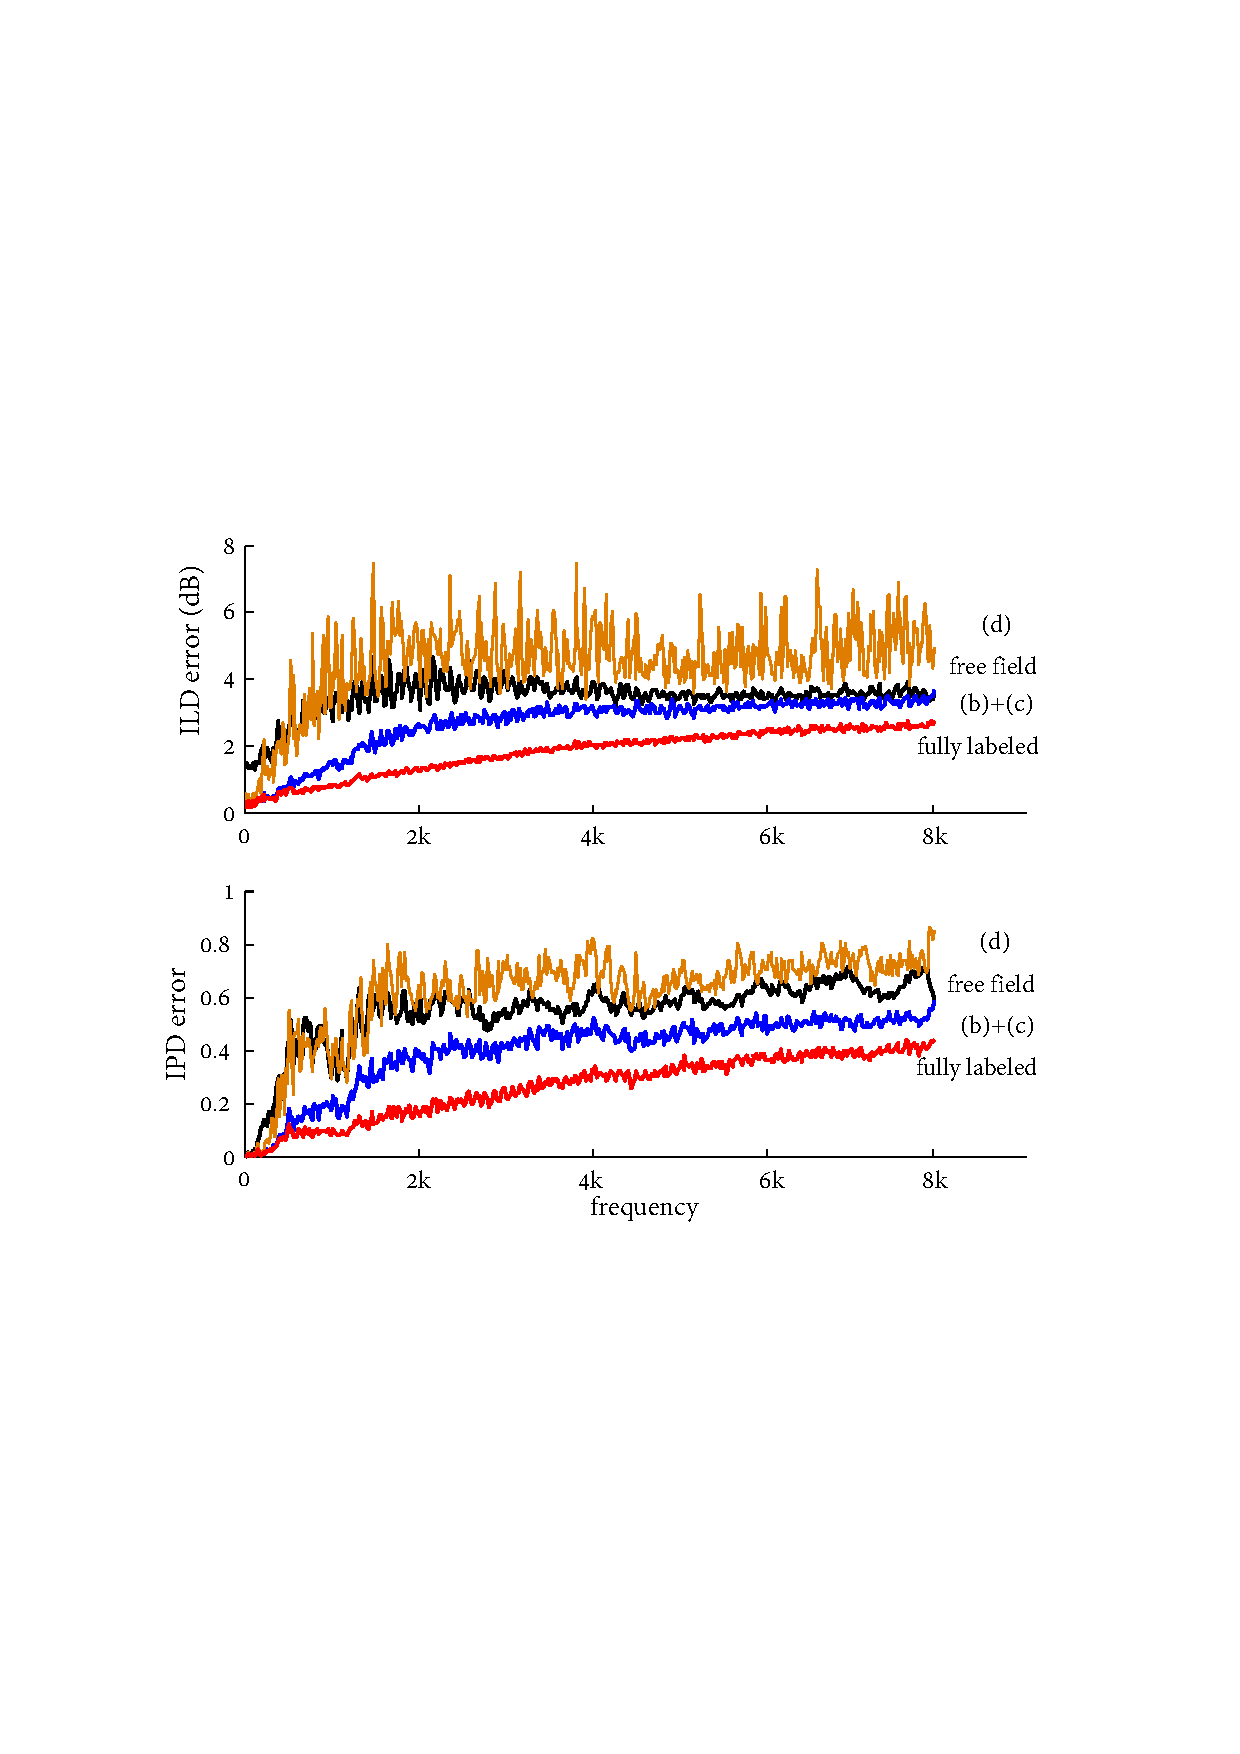
\includegraphics[width=8.5cm]{fig3_err_freq.pdf}}
    \caption{ILD/IPD mean prediction errors along frequency for network (d), free field model, network (b)+(c) and network trained with fully labeled data.}
    \label{fig3}
\end{figure}

The prediction errors clearly increase with frequency and become relatively stable in the high frequencies. One possible reason could be that the RTFs vary more rapidly with respect to pose changes in the high frequencies as can be concluded from the free field model (3), while the slow-varying RTFs in the low frequencies are easier to be captured by the neural networks. The network trained with fully labeled data achieves the lowest mean prediction errors as expected, with 1.80$\pm$0.09 dB in ILD and 0.26$\pm$0.02 in IPD. It is significantly better than other setups where only few training data are labeled. The unlabeled RTFs function differently in different architectures. The (b)+(c) network performs much better than the free field model, while the intuitive encoder-decoder setup (a)+(c), that relies on the same training data, fails to give good predictions. To see how the unlabeled samples help, we investigate the encoder networks in terms of pose localization performance. The root mean squared error (RMSE) between the encoder outputs and the true source poses are computed. For encoder (a), the localization RMSEs are 13.08$^{\circ}$ in azimuth and 8.74$^{\circ}$ in elevation. For the encoder (b) with manifold regularization, the results are 2.94$^{\circ}$ and 2.08$^{\circ}$, respectively, which are quite accurate pose predictions considering that the labeled samples are 10$^{\circ}$ away in distance. It can be interpreted as that the encoders provide the unlabeled RTFs with noisy pose labels. Additional experiments show that the manifold regularized encoder even slightly outperforms the recently proposed MRL in same localization tasks.

The decoder network (d) with regularization has similar prediction errors in frequencies below 1 kHz compared with the free field model but its performance falls behind in the high frequencies. It is concluded that the $l_2$ norm used in (9) to measure the affinity between RTFs is not proper since it ignores the angle of the high-dimensional vector, though the $l_2$ norm clearly makes more sense for measuring the poses.

% table
\begin{table}[tb]
\caption{Summarization of frequency averaged ILD/IPD prediction errors (mean$\pm$CI bound) and SBF (dB).}
\label{table:1}
\begin{center}
\begin{tabular}{|l|c|c||c|}
  \hline
                       & ILD error & IPD error & SBF \\ \hline
   (a)+(c)    & 4.05$\pm$0.23 & 0.64$\pm$0.03  &  -0.60\\ \hline
   (d)        & 3.94$\pm$0.20 & 0.61$\pm$0.03   &  -0.35\\ \hline
   free field model & 3.47$\pm$0.16 & 0.55$\pm$0.03 & 0.69\\ \hline
   (b)+(c)    & 2.67$\pm$0.13 & 0.39$\pm$0.02    &  2.04   \\ \hline
   fully labeled & 1.80$\pm$0.09 & 0.26$\pm$0.02 &  3.19 \\ \hline
\end{tabular}
\end{center}
\end{table}

%\begin{figure}[tb]
%    \centering
%    \centerline{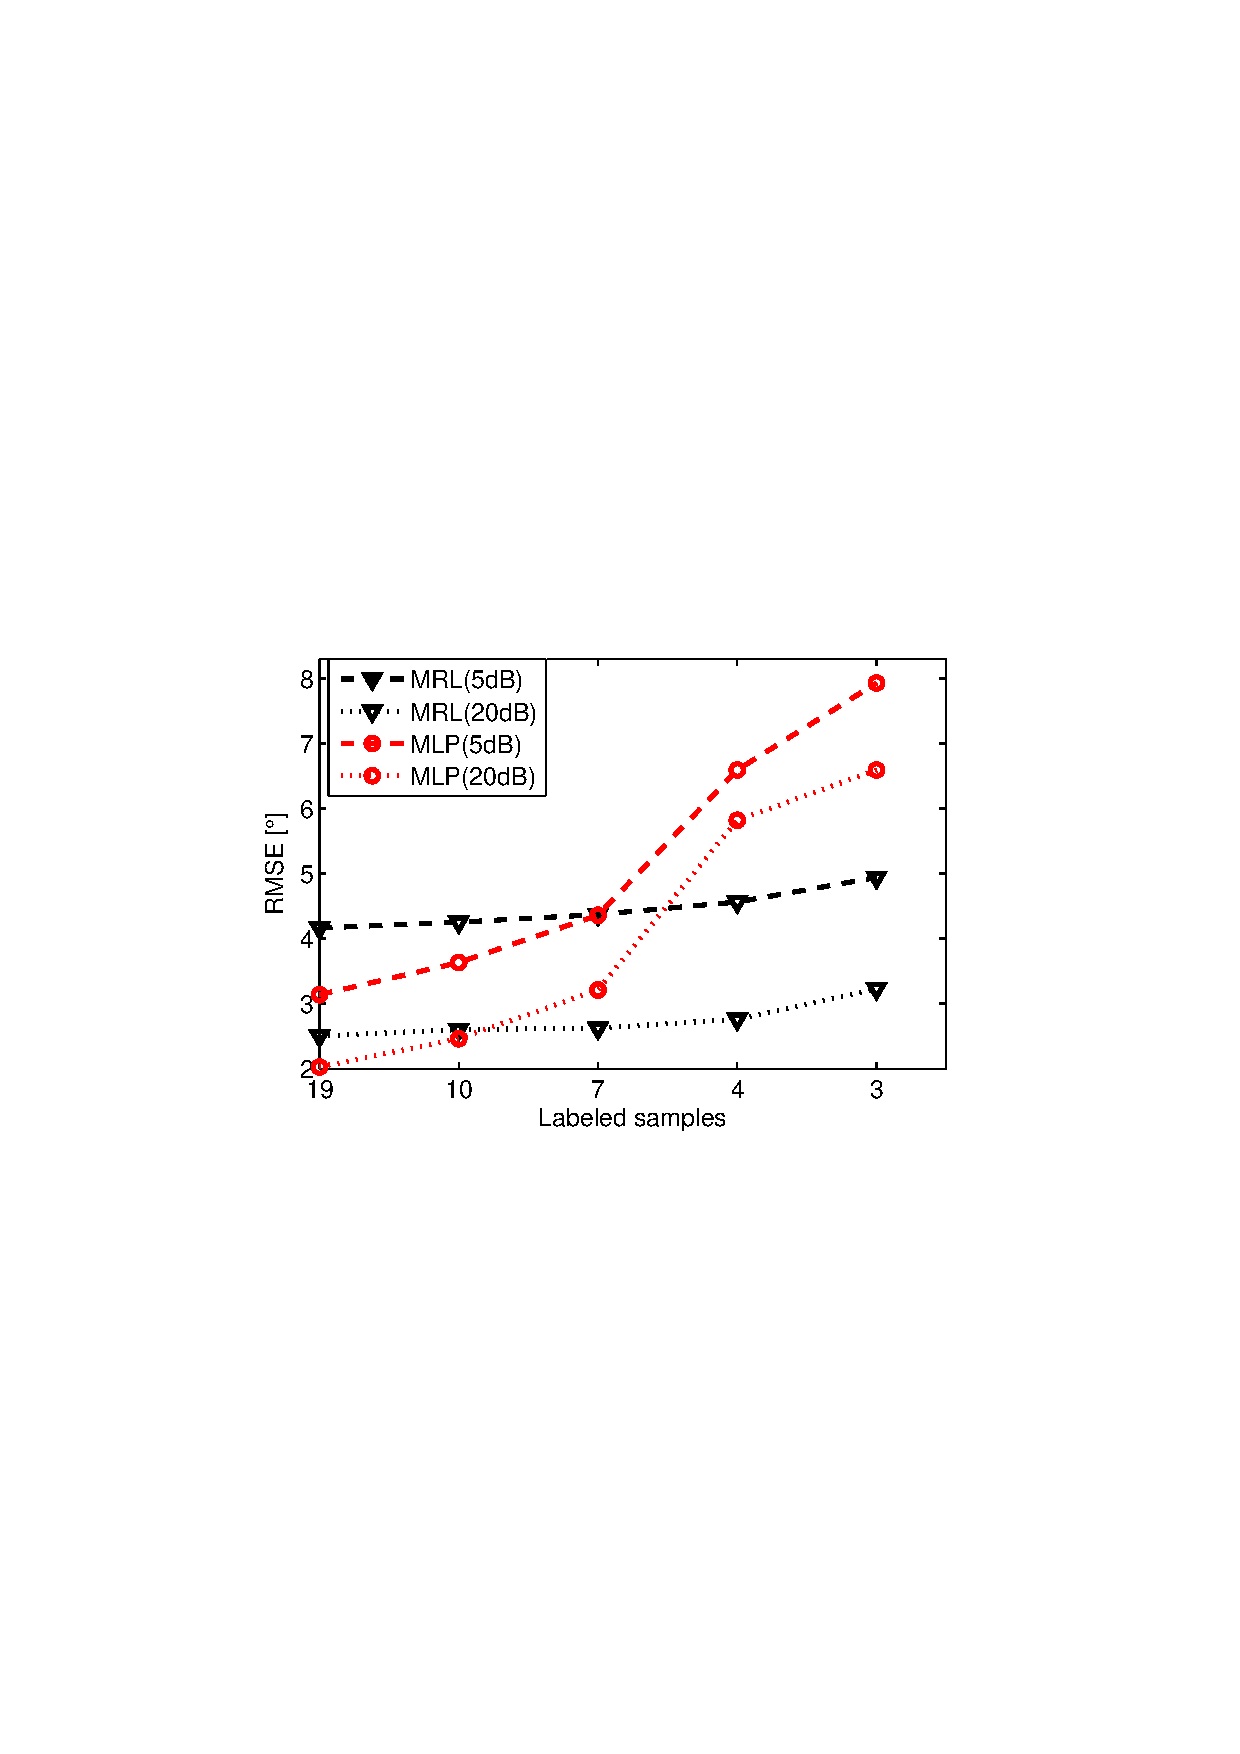
\includegraphics[width=8.0cm]{fig4_mrl.pdf}}
%    \caption{Localization RMSE of the encoder network (b) compared with MRL.}
%    \label{fig4}
%\end{figure}


\subsection{Further analysis}

It is commonly acknowledged that learning based methods would perform better with more labeled training data and suffer performance loss in mismatched test conditions. So these aspects are not further investigated here. Instead we evaluate the generated RTFs in a specific application, the generalized sidelobe canceller (GSC)~\cite{gannot2001signal}, that requires RTF in the implementation of a blocking matrix to provide the reference noise signal. A frequency domain signal blocking factor (SBF) is first defined as:
\begin{equation}\label{eq:sbf}
  \text{SBF}=10\text{log}_{10}\frac{\sum_{n,k} ||A_1(n,k)||^2}{\sum_{n,k} ||A_2(n,k)-H({\bf p},k)A_1(n,k)||^2}
\end{equation}
where the denominator denotes the energy of the leakage signal. SBF indicates the ability to block the first-channel source image in the second microphone and its value correlates negatively with signal distortion.

The SBF scores of different methods are given in Table~1. The results are consistent with the mean prediction errors, with the fully labeled setup scoring the best (3.19 dB), the (b)+(c) network outperforming the free field model and the simple (a)+(c) the scoring the worst (-0.60 dB). The negative score means that the generated RTF is not helpful at all.

Meanwhile the generated RTF should be considered as prior information obtained from the source pose only and further performance benefits are expected if it is incorporated with the observations to achieve maximum a posterior RTF estimation.


\section{CONCLUSIONS}
\label{sec:con}

We considered the RTF inverse regression task from a practical perspective where partial training data is labeled and introduced the semi-supervised learning method. Several possible architectures were discussed. The proposed encoder with manifold regularization and decoder architecture outperformed the free field model, in terms of both mean prediction error and signal blocking ability in the GSC application. Direct smoothness regularization on the high-dimensional RTF vector didn't work well, and we concluded that the unlabeled RTFs were indeed necessary in the final performance. Incorporating and evaluating the generated prior RTFs in other applications is some work worth further investigation.

% Below is an example of how to insert images. Delete the ``\vspace'' line,
% uncomment the preceding line ``\centerline...'' and replace ``imageX.ps''
% with a suitable PostScript file name.
% -------------------------------------------------------------------------
%\begin{figure}[htb]

%\begin{minipage}[b]{1.0\linewidth}
%  \centering
%  \centerline{\includegraphics[width=8.5cm]{image1}}
%  \vspace{2.0cm}
%  \centerline{(a) Result 1}\medskip
%\end{minipage}
%
%\begin{minipage}[b]{.48\linewidth}
%  \centering
%  \centerline{\includegraphics[width=4.0cm]{image3}}
%  \vspace{1.5cm}
%  \centerline{(b) Results 3}\medskip
%\end{minipage}
%\hfill
%\begin{minipage}[b]{0.48\linewidth}
%  \centering
 % \centerline{\includegraphics[width=4.0cm]{image4}}
%  \vspace{1.5cm}
 % \centerline{(c) Result 4}\medskip
%\end{minipage}
%
%\caption{Example of placing a figure with experimental results.}
%\label{fig:res}
%
%\end{figure}


% To start a new column (but not a new page) and help balance the last-page
% column length use \vfill\pagebreak.
% -------------------------------------------------------------------------
%\vfill
%\pagebreak

%\section{COPYRIGHT FORMS}
%\label{sec:copyright}
%You must submit your fully completed, signed IEEE electronic copyright release
%form when you submit your paper. We {\bf must} have this form before your paper
%can be published in the proceedings.
%\vfill\pagebreak

%\newpage

% References should be produced using the bibtex program from suitable
% BiBTeX files (here: strings, refs, manuals). The IEEEbib.bst bibliography
% style file from IEEE produces unsorted bibliography list.
% -------------------------------------------------------------------------
\bibliographystyle{IEEEbib}
\bibliography{refs}

\end{document}
